\documentclass{beamer}	
\usecolortheme{wolverine}

\setbeamertemplate{caption}{\raggedright\insertcaption\par}

\usepackage{tabularx}
\usepackage{booktabs}
\usepackage{multirow}
\newcolumntype{C}{>{\centering\arraybackslash}X}
\usepackage{proof}
\usepackage{amsmath}
\usepackage{wasysym}
\usepackage{tikz}
\usetikzlibrary{arrows.meta,positioning,matrix}

\newcommand{\term}[1]{\texttt{#1}}

\title{Intuitionistic Logic}
\author{K. Kogkalidis}
\institute{Logic \& Language 2020}

% exercise ideas: show lambda term difference between tuple reversals

\begin{document}
\date{}
\maketitle

\begin{frame}{Intuitionism}

\begin{minipage}[t]{0.3\textwidth}
	\begin{figure}
	\includegraphics[scale=0.85]{Brouwer}
	\caption{L. E. J. Brouwer}
	\end{figure}
\end{minipage}%
\begin{minipage}[t]{0.7\textwidth}
	\begin{block}{Main Tenets}
	\begin{itemize}
		\item Mathematical truth is subjective rather than fundamental
		\item Proof is a process of construction rather than discovery
		\item A mathematical object exists if it can be constructed
	\end{itemize}
	\end{block}
\end{minipage}
\vfill


\begin{minipage}[t]{0.7\textwidth}
	\begin{block}{Intuitionistic Logic}
		A different formal model to capture the notion of Intuitionistic Truth, which is stricter
		than Classical Truth
	\end{block}
\end{minipage}%
\begin{minipage}[t]{0.3\textwidth}
\begin{figure}
\includegraphics[scale=0.175]{Heyting}
\caption{Arend Heyting}
\end{figure}
\end{minipage}
\end{frame}


\begin{frame}{Intuitionistic Logic vs Classical Logic}
	\alert{CL}:
	\begin{itemize}
		\item Propositions are either true or false
		\item[] \quad 
			\small{\alert{Law of exluded middle}:
				$\top \to (A \vee \neg A)$
			}
		\item Negation is Falsity
		\item[] \quad 
			\small{\alert{Double Negation Elimination}:
				$\neg (\neg A) \to A$
			}
	\end{itemize}
	\vfill
	
	\alert{IL}:
	\begin{itemize}
		\item Propositions are \textit{proven} (true) or \textit{unproven} (anything)
		\item Negation is refutability
	\end{itemize}
	\vfill
	
	\begin{block}{Consequence}
		IL is a \alert{weaker} logic, disallowing proof by contradiction
	\end{block}	
	
\end{frame}

% Interpretation of formulas:
%	True/False  vs. Proof/No proof (inhabited/uninhabited)
%	Negation: Falsity	vs Negation: Counter-evidence
%

\begin{frame}{Basic Definitions: Proposition}

	\begin{block}{Propositions}
		Let $\mathcal{C}$ a set of \textit{propositional constants}.
		The \textit{propositions} (formulas) $\mathcal{P}$ of IL are:
		\[
		\mathcal{P} := \mathcal{C}  \ | \ \mathcal{P}_1 \to \mathcal{P}_2 \ | \ \mathcal{P}_1 \times \mathcal{P}_2 \
		| \ \mathcal{P}_1 + \mathcal{P}_2
		\]
	
	where:
	\begin{itemize}
		\item[$\to$] is read as ``implies''
		\item[$\times$] is read as ``and''
		\item[$+$] is read as ``or''
	\end{itemize}
	\end{block}
	
	\begin{flushright}
		\small
		We will denote propositional constants by $A, B, C, \dots$
	\end{flushright}
\end{frame}
% give some examples, talk about operator priority

\begin{frame}{Basic Definitions: Assumption \& Judgement}
	\begin{block}{Assumptions}
		An \textit{assumption} (context) $\mathcal{A}$ is a sequence of zero or more propositions:
		\[
			\mathcal{A} := \left( \right) \ | \ \mathcal{A}, \mathcal{P}
		\]
	\end{block}
	
	\begin{flushright}
		\small
		We will denote assumptions by $\Gamma, \Delta, \Theta, \dots$
	\end{flushright}
	
	\begin{block}{Judgement}
		A \textit{judgement} $\mathcal{J}$ is a statement $\mathcal{A} \vdash \mathcal{P}$
	\end{block}
	
	\begin{flushright}
		\small 
		Read as ``\textit{from assumptions $\mathcal{A}$, one can conclude proposition $\mathcal{P}$}''
	\end{flushright}
\end{frame}

\begin{frame}{Basic Definitions: Rule}	
	\begin{block}{Rule}
	A \textit{rule} is a statement consisting of zero or more \alert{premises} $\mathcal{J}_1, \dots \mathcal{J}_n$ and a \alert{conclusion} $\mathcal{J}_c$:
	\[
		\infer[]{\mathcal{J}_c}{
		\mathcal{J}_1 
		&
		\dots 
		&
		\mathcal{J}_n
		}
	\]
	\end{block}
	
	\begin{flushright}
		\small
		If every $\mathcal{J}_i$ is derivable (has a proof), we can derive $\mathcal{J}_c$
	\end{flushright}

	\begin{block}{Axiom Rule}
	From any formula $A$, one can conclude itself:
	\[
		\infer[Ax]{A \vdash A}{}
	\]
	
	\end{block}

\end{frame}

\begin{frame}{Logical Rules}
	Each logical connective $\to, \times, +$ has rules for its \textit{introduction} and \textit{elimination}:
	\pause
	\[
	\infer[\to I]{\Gamma \vdash A \to B}{\Gamma, A \vdash B}
	\quad
    \infer[\to E]{\Gamma, \Delta \vdash B}
	{\Gamma \vdash A \to B
	&
	\Delta \vdash A}
	\]
	\pause
	
	\[
	\infer[\times I]{\Gamma, \Delta \vdash A \times B}{
		\Gamma \vdash A
		&
		\Delta \vdash B
	}
	\quad
    \infer[\times E]{\Gamma, \Delta \vdash C }
	{\Gamma \vdash A \times B
	&
	\Delta, A, B \vdash C}
	\]
	\pause
	
	\vfill
	\[
	\infer[+E]{\Gamma, \Delta \vdash C}{
	\Gamma \vdash A + B
	& 
	\Delta, A \vdash C
	&
	\Delta, B \vdash C	
	}
	\]
	
	\[
	\begin{array}{cc}
	\infer[+I_1]{\Gamma \vdash A + B}{
	\Gamma \vdash A
	} 
	&
	\infer[+I_2]{\Gamma \vdash A + B}{
	\Gamma \vdash B}
	\end{array}
	\]
\end{frame}

\begin{frame}{Structural Rules}
	The $,$ of IL assumptions is \textit{commutative}:
	\[
		\infer[\text{Exchange}]{\Gamma, \Delta \vdash A}{\Delta, \Gamma \vdash A}
	\]
	\vfill
	
	IL propositions are free to \textit{discard} and \textit{replicate}:
	\[
	\begin{array}{ccc}
		\infer[\text{Contraction}]{\Gamma, A \vdash B}{\Gamma, A, A \vdash B}
	&
	&
		\infer[\text{Weakening}]{\Gamma, A \vdash B}{\Gamma \vdash B}
	\end{array}
	\]
\end{frame}


\begin{frame}{Example: Identity Function}
	\small
	\[
		\infer[\visible<2->{\to I}]{ \ \vdash A \to A}{
		\visible<2->{
			\infer[Ax]{A \vdash A}{}
		}
		}
	\]
\end{frame}


\begin{frame}{Example: Tuple Reversal}
	\small
	\[
		\infer[\visible<2->{\times E}]{A\times B \vdash B\times A}{
		\visible<2->{
			\infer[\visible<3->{Ax}]{A \times B \vdash A \times B}{}
			& 
			\infer[\visible<4->{Ex}]{A, B \vdash B\times A}{
			\visible<4->{
				\infer[\visible<5->{\times I}]{B, A \vdash B\times A}{
				\visible<5->{
					\infer[Ax]{B \vdash B}{}
					&
					\infer[Ax]{A \vdash A}{}
				}}
			}}
		}}
	\]

\end{frame}

\begin{frame}{Example: Function Composition}
	\small
	\[
		\infer[\visible<2->{\to I}]{A\to B, B\to C \vdash A\to C}{
		\visible<2->{
			\infer[\visible<3->{\text{Ex}}]{A\to B, B\to C, A \vdash C}{
			\visible<3->{
				\infer[\visible<4->{\to E}]{B\to C, A, A\to B \vdash C}{
					\visible<4->{
					\infer[Ax]{B \to C \vdash B \to C}{}
					}
					&
					\visible<5->{
					\infer[\visible<6->{\text{Ex}}]{A, A\to B \vdash B}{
					\visible<6->{
						\infer[\visible<7->{\to E}]{A\to B, A \vdash B}{
						\visible<7->{
							\infer[Ax]{A\to B \vdash A \to B}{}
							&
							\infer[Ax]{A \vdash A}{}
						}
						}
					}
					}
				}
				}
			}
			}
		}
		}
	\]
\end{frame}


%\begin{frame}{Example: Tuple Reversal}
%	\small
%	\[
%		\infer[\visible<2->{\text{C}}]{A\times B \vdash B \times A}{
%		\visible<2->{
%			\infer[\visible<3->{\times I}]{A\times B, A\times B \vdash B\times A}{
%			\visible<3->{
%				\infer[\visible<4->{\times E}]{A\times B \vdash B}{
%				\visible<4->{
%					\infer[Ax]{A\times B \vdash A \times B}{}
%					&
%					\infer[\visible<5->{\text{Ex}}]{A, B \vdash B}{
%					\visible<5->{
%						\infer[\visible<6->{\text{\small W}}]{B, A \vdash B}{
%						\visible<6->{
%							\infer[Ax]{B \vdash B}{}
%						}
%						}
%					}
%					}
%				}
%				}
%				&
%				\infer[\visible<7->{\times E}]{A\times B \vdash A}{
%				\visible<7->{
%					\infer[Ax]{A\times B \vdash A \times B}{}
%					&
%					\infer[\text{W}]{A, B \vdash A}{
%						\infer[Ax]{A \vdash A}{}
%					}
%				}
%				}
%			}
%			}
%		}
%		}
%	\]
%\end{frame}

\begin{frame}{Example: Currying}
	\small
	\[
		\infer[\visible<2->{\to I}]{(A \times B) \to C \vdash A \to B \to C}{
		\visible<2->{
			\infer[\visible<3->{\to I}]{(A\times B) \to C, A \vdash B \to C}{
			\visible<3->{
				\infer[\visible<4->{\to E}]{(A\times B)\to C, A, B \vdash C}{
				\visible<4->{
					\infer[Ax]{(A\times B)\to C \vdash (A\times B) \to C}{}
					&
					\infer[\visible<5->{\times I}]{A, B \vdash A \times B}{
					\visible<5->{
						\infer[Ax]{A \vdash A}{}
						&
						\infer[Ax]{B \vdash B}{}
					}
					}
				}
				}
			}
			}
		}
		}
	\]
\end{frame}

\begin{frame}{Proof Normalization}
	A single judgement may have many distinct proofs:
	\begin{itemize}
		\item[\smiley{}] ``Morally'' distinct: different construction methods
		\item[\frownie{}] Redundant elongations due to chaining I/E or C/W rules
	\end{itemize}
	\vfill
	
	\small
	\[
	\infer[]{\dots}{
		\infer[\textcolor{red}{\to E}]{A\to B, A \vdash B}{
			\infer[\textcolor{red}{\to I}]{A \to B \vdash A \to B}{
				\infer[]{\textcolor{red}{A\to B, A \vdash B}}{\dots}
			}
			&
			\infer[Ax]{A\vdash A}{}
		}
	}
	\]

\end{frame}


\begin{frame}{Curry-Howard Correspondence}
	\begin{minipage}[b]{0.33\textwidth}
		\begin{figure}
		\includegraphics[width=0.66\textwidth]{Curry}
		\caption{Haskell Curry}
		\end{figure}
	\end{minipage}%
	\begin{minipage}[b]{0.33\textwidth}
		\begin{figure}
		\includegraphics[width=0.66\textwidth]{Howard}
		\caption{William Howard}
		\end{figure}
	\end{minipage}%
	\begin{minipage}[b]{0.33\textwidth}
		\begin{figure}
		\includegraphics[width=0.66\textwidth]{deBruijn}
		\caption{Nicolas de Bruijn}
		\end{figure}
	\end{minipage}
	
	\vfill
	
	\begin{minipage}[b]{0.66\textwidth}
	\begin{block}{Curry-Howard Correspondence}
		Intuitionistic Logic describes a model of computation, known as
		the \alert{simply-typed $\lambda$-calculus $\lambda^\to$}
		
%		\centering
%\textbf{the simply typed $\lambda$-calculus}
	\end{block}
	\end{minipage}%
	\begin{minipage}{0.33\textwidth}
		\begin{figure}
		\includegraphics[width=0.66\textwidth]{Church}
		\caption{Alonzo Church}
		\end{figure}
	\end{minipage}

\end{frame}


\begin{frame}{Propositions as Types}
    \newcolumntype{C}{>{\centering\arraybackslash}X}

	\footnotesize
	\centering
	\begin{tabularx}{0.825\textwidth}{@{}CC}
	\textbf{Logic} & \textbf{Programming}\\	
	\toprule
	Proposition & Type \\
	Proof & Algorithm \\
	Provability & Type Inhabitation \\ 
	Proof Normalization & $\beta$-reduction \\
	\midrule
	Propositional Constant & Primitive Type \\
	Axiom & Variable Instantiation \\
	Logical Connectives & Type Operators \\ 
	Introduction Rules & Type Constructors \\
	Elimination Rules & Type Destructors \\
	Implication Introduction & Function Abstraction \\
	Implication Elimination & Function Application \\
	\multicolumn{2}{c}{\dots} \\
%	\multirow{2}{*}{\textbf{Metric} (\%)} & \multicolumn{5}{c}{\textbf{Beam Size} $\vec\beta$} \\ 
	\end{tabularx} 	
\end{frame}

\begin{frame}{Terms of the simply typed $\lambda$-calculus}
	\small
	
	Each proposition($\equiv$ \textit{type}) $\mathcal{P}$ is assigned a unique \textit{term} (name) $\mathcal{T}$:
	\[
		\mathcal{T}: \mathcal{P}
	\]
	\vfill
	
	Assumptions $\mathcal{A}$ are now interpreted as a \textit{typing environment}:
	\[
		\mathcal{A} := ( ) \ | \ \mathcal{A}, \mathcal{T}: \mathcal{P}
	\]
	
\end{frame}

\begin{frame}{Terms of the simply typed $\lambda$-calculus}
	Let $\mathcal{V}$ a set of \textit{primitive terms} (variables).

	\begin{flushright}
		\small
		We will denote primitive terms by \term{x, y, z, \dots}
	\end{flushright}

	The terms $\mathcal{T}$	of the simply typed $\lambda$-calculus then are:

	\begin{align*}
		\mathcal{T} :=& \ 
					\visible<2->{\mathcal{V}}
					\visible<3->{\ | \ \mathcal{T}(\mathcal{T})} 
					\visible<4->{\ | \ \lambda\mathcal{T}.\mathcal{T}
					& \textit{\small Implication-Only}} \\
					\visible<5->{& \ | \ (\mathcal{T}, \mathcal{T})}
					\visible<6->{ \ | \ \term{case $\mathcal{T}$ of $(\mathcal{T}, \mathcal{T}) \to \mathcal{T}$}
					& \textit{\small /w Product}} \\
					\visible<7->{& \ | \ \term{inl}(\mathcal{T}) \ | \ \term{inr}(\mathcal{T})} \\
					\visible<8->{& \ | \ \term{case s of inl(x)} \to \term{w; inr(y)} \to \term{z}
					& \textit{\small /w Co-product}}
	\end{align*}

	\vfill
	\small

	\alt<1>{
	% frame 1
	}{
	\alt<2>{
	% frame 2
	
	\[
		\infer[Ax]{\term{x}: A \vdash \term{x}: A}{}
	\]
	}
	{
	\alt<3>{
	% frame 3
	
	\[
		\infer[\to E]{\Gamma, \Delta \vdash: \term{f(x)}\footnote{Can also be written \term{f x}}: B}{
			\Gamma \vdash \term{f}:A \to B
			&
			\Delta \vdash \term{x}: A
		}
	\]
	}
	{
	\alt<4>{
	% frame 4
	
	\[
		\infer[\to I]{\Gamma \vdash \lambda \term{x.f}: A \to B}{
			\Gamma, \term{x}:A \vdash \term{f}: B
		}
	\]
	}
	{
	\alt<5>{
	% frame 5
	
	\[	
		\infer[\times I]{\Gamma, \Delta \vdash \term{(x, y)}: A \times B}{
		\Gamma \vdash \term{x}: A
		&
		\Delta \vdash \term{y}: B
		}
	\]
	}
	{
	\alt<6>{
	% frame 6
	
	\[
	    \infer[\times E]{\Gamma, \Delta \vdash 
	    \term{case s of (x, y)} \to \term{w}:
	    C }{
	    	\Gamma \vdash \term{s}: A \times B
			&
			\Delta, \term{x}: A, \term{y}: B \vdash \term{w}: C
		}
	\]
	}
	{
	\alt<7>{
	% frame 7
	
	\[
		\begin{array}{cc}
			\infer[+I_1]{\Gamma \vdash \term{inl(x)}: A + B}{
				\Gamma \vdash \term{x}: A
			} 
			&
			\infer[+I_2]{\Gamma \vdash \term{inr(x)}: A + B}{
				\Gamma \vdash \term{x}: B
			}
		\end{array}
	\]
	}
	{
	\alt<8>{
	
	\[
		\infer[+E]{\Gamma \vdash 
		\term{case s of inl(x)} \to \term{w; inr(y)} \to \term{z}:
		C}{
			\Gamma \vdash \term{s}: A + B
			&	 
			\Delta, \term{x}:A \vdash \term{w}:C
			&
			\Delta, \term{y}:B \vdash \term{z}:C	
	}
	\]
	}
	{
	}}}}}}}}
\end{frame}


\begin{frame}{Terms: Uniqueness \& Structural Rules}

	Variable names must be \alert{unique} for each distinct formula instantiation in a proof!

	\[
		\infer[\text{Contraction}]{\Gamma, \term{x}: A \vdash
		\term{u[x/y,x/z]}: B}{
			\Gamma, \term{y}: A, \term{z}: A \vdash \term{u}:B
		}
	\]
	
	\[
		\infer[\text{Weakening}]{\Gamma, \term{x}:A \vdash \term{u}:B}{\Gamma \vdash \term{u}:B}
	\]
\end{frame}

\begin{frame}{Example: Identity Function Revisited}
	\[
		\infer[\to I]{\alt<3->{\textcolor{blue}{\ \vdash \lambda\term{x.x}: A \to A}}{\ \vdash A\to A}}{
			\infer[Ax]{\alt<2->{\textcolor{blue}{\term{x}: A \vdash \term{x}: A}}{A \vdash A}}{}
		}
	\]
\end{frame}


\begin{frame}{Example: Function Composition Revisited}
	\footnotesize
	\[
		\infer[\to I]{\alt<6->{\textcolor{blue}{\term{f}: A\to B, \term{g}: B\to C \vdash \lambda\term{x.(g (f x))}:A\to C}}{A\to B, B\to C \vdash A\to C}}{
			\infer[\text{Ex}]{\alt<5->{\textcolor{blue}{\term{f}: A\to B, \term{g}: B\to C, \term{x}: A \vdash \term{g (f x)}: C}}{A\to B, B\to C, A \vdash C}}{
				\infer[\to E]{\alt<4->{\textcolor{blue}{\term{g}: B\to C, \term{x}: A, \term{f}: A\to B \vdash \term{g (f x)}: C}}{B\to C, A, A\to B \vdash C}}{
					\infer[Ax]{\alt<2->{\textcolor{blue}{\term{g}: B\to C \vdash \term{g}:B\to C}}{B \to C \vdash B \to C}}{}
					&
					\infer[\text{Ex}]{\alt<4->{\textcolor{blue}{\term{x}: A, \term{f}: A\to B \vdash \term{f x}: B}}{A, A\to B \vdash B}}{
						\infer[\to E]{\alt<3->{\textcolor{blue}{\term{f}: A \to B, \term{x}: A \vdash \term{f x}: B}}{A\to B, A \vdash B}}{
							\infer[Ax]{\alt<2->{\textcolor{blue}{\term{f}: A\to B \vdash \term{f}: A\to B}}{A\to B \vdash A \to B}}{}
							&
							\infer[Ax]{\alt<2->{\textcolor{blue}{\term{x}: A \vdash \term{x}: A}}{A \vdash A}}{}
						}
					}
				}
			}
		}
	\]
\end{frame}

\begin{frame}{Term Equivalence \& Reduction}
	\small 
	
	\begin{itemize}
		\item \alert{$\alpha$-conversion} Changing the name of bound variables
		\[
			\lambda x.x \stackrel{\alpha}{\equiv} \lambda y.y
		\]
		\item \alert{Substitution} Changing the name of free variables
		\[
			(f\  g)(\lambda x.(x \ g))[h/g] = (f\ h)(\lambda x.(x \ h))	
		\]
		\item \alert{$\eta$-reduction} Simplifying an abstraction if the abstracted variable does not occur free in the function body
		\[
			\lambda x.f \ x \stackrel{\eta}{\equiv} f \ \text{($x$ does not occur in $f$)}
		\]
		\item \alert{$\beta$-reduction} Removing any applicable abstraction
		\[
			(\lambda x.g)(y) \Longrightarrow g[x/y]
		\]
	\end{itemize}
	
	\begin{block}{Proof Normalization $\equiv$ Term Reduction}
		\begin{itemize}
			\item Church-Rosser: order of term reduction rules is irrevelant
			\item Subject Reduction: term reduction rules on well-typed terms produce well-typed terms
		\end{itemize}
	\end{block}
\end{frame}

\begin{frame}{Proof Normalization \& Term Reduction ($\to$)}
	\small 
	
	\[
		\begin{array}[t]{@{}ccc}
			\infer[\textcolor{red}{\to E}]{\Gamma, \Delta \vdash (\lambda\term{x.u})(\term{t}): B}{
				\infer[\textcolor{red}{\to I}]{\Gamma \vdash \lambda\term{x.u}: A \to B}{
					\infer=[]{\Gamma, \term{x}: A \vdash \term{u}: B}{
						\infer*[]{\Gamma, \term{x}: A, \dots \vdash \term{u}: B}{
							\infer[]{\term{x}: A \vdash \term{x}: A}{}
							\
							\dots
						}
					}
				}
				&
				\infer[]{\Delta \vdash \term{t}: A}{\vdots}
			}		
			&
			\Rightarrow
			&
			\infer=[]{\Gamma, \Delta \vdash \term{u}: B}{
				\infer*[]{\Gamma, \Delta, \dots \vdash \term{u}: B}{
					\infer*[]{\Delta \vdash \term{t}: A}{}
					\
					\dots
				}
			}
		\end{array}
	\]	
	
	\alert{
	\[
		(\lambda\term{x.u})(\term{t}) \Longrightarrow u[t/x]
	\]
	}
	\begin{flushright}
		$\beta$-reduction
	\end{flushright}

\end{frame}

\begin{frame}{Proof Normalization \& Term Reduction ($\times$)}
	\small 
	\[
	\begin{array}{c}
		\infer[\textcolor{red}{\times E}]{\Gamma, \Delta, \Theta \vdash C}{
			\infer[\textcolor{red}{\times I}]{\Gamma, \Delta \vdash \term{(t, u)}: A \times B}{
				\infer*[]{\Gamma \vdash \term{t}: A}{}
				&
				\infer*[]{\Delta \vdash \term{u}: B}{}
			}
			&
			\infer=[]{\Theta, A, B \vdash C}{
				\infer*[]{\Theta, A, \dots, B, \dots \vdash \term{v}: C}{
				\infer[]{\term{x}: A \vdash \term{x}: A}{}
				& 
				\dots
				&
				\infer[]{\term{y}: B \vdash \term{y}: B}{}
				}
			}
		}
		\\
		{\left\Downarrow\vbox to 1em{}\right.\kern-\nulldelimiterspace}\\
		\infer=[]{\Gamma, \Delta, \Theta \vdash \term{v}: C}{
			\infer*[]{\Gamma, \dots, \Delta, \dots, \Theta \vdash \term{v}: C}{
				\infer*[]{\Gamma \vdash \term{t}: A}{}
				&
				\dots
				&
				\infer*[]{\Delta \vdash \term{u}: B}{}
			}
		}
	\end{array}
	\]

	\alert{
	\[
		\term{case (t,u) of (x,y)}\to \term{v} \Longrightarrow v[t/x, u/y]
	\]
	}
\end{frame}

\begin{frame}{Proof Normalization \& Term Reduction ($+$)}
	\small
	\[
		\begin{array}{c}
			\infer[\textcolor{red}{+ E}]{\Gamma, \Delta \vdash \term{case inr(t) of inl(x)}\to\term{v}; \term{inr(y)}\to\term{w}: C}{
				\infer[\textcolor{red}{+ I_2}]{\Gamma \vdash \term{inr(t)}: A + B}{
					\infer*[]{\Gamma \vdash \term{t}: B}{}
				}
				&
				\infer=[]{\Delta, \term{x}: A \vdash \term{v}: C}{
					\infer*[]{\Delta, \term{x}: A \dots \vdash \term{v}: C}{
					\infer[]{\term{x}: A \vdash \term{x}: A}{}
					}
				}
				&
				\infer=[]{\Delta, \term{y}: B \vdash \term{w}: C}{
					\infer*[]{\Delta, \term{y}: B \dots \vdash \term{w}: C}{
						\infer[]{\term{y}: B \vdash \term{y}: B}{}
					}
				}
			}
			\\
			{\left\Downarrow\vbox to 1em{}\right.\kern-\nulldelimiterspace}\\
			\infer=[]{\Gamma, \Delta \vdash \term{w}: C}{
				\infer*[]{\Gamma, \dots, \Delta, \dots \vdash \term{w}: C}{
					\infer*[]{\Gamma \vdash \term{t}: B}{}
					&
					\dots
				}
			}
		\end{array}
	\]

	\alert{
	\[
		\term{case inr(t) of inl(x)}\to\term{v}; \term{inr(y)}\to\term{w} \Longrightarrow w[t/y]
	\]
	}

	\vfill
	\begin{flushright}
		Similarly for $+ I_1$
	\end{flushright}
	% ex:
	% B x D, A -> C x B -> C |- C
\end{frame}


\begin{frame}[fragile]{Beyond simple types: the $\lambda$-Cube}
	\small
	
	Three axes of extension:
	\begin{itemize}
		\item[$\lambda2$] Terms can depend on types 
		\[
		\vcenter{\infer[]{\Gamma \vdash \Lambda \term{a.t}: \Pi a.A  }{\Gamma \vdash \term{t}: A}}
		\]
		\item[$\lambda\Pi$]	Types can depend on terms
		\[
			\infer[]{\Gamma \vdash \Pi\term{x.A.B}: *}{\Gamma, \term{x}: A \vdash \term{B}: *}
		\]
		\item[$\lambda\underline\omega$] Types can depend on types
		\[
			\lambda A: *.(A\to B)\to(B\to B \to B)\to B
		\]
	\end{itemize}	
	
	\centering
		
		\hspace{80pt}
		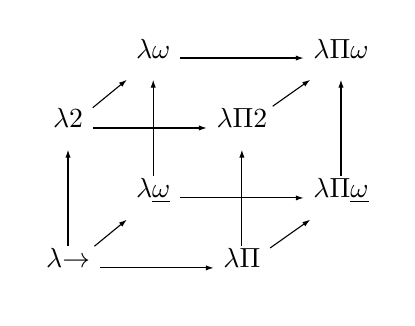
\begin{tikzpicture}
		\matrix (m) [matrix of math nodes,
		row sep=1em, column sep=1em,
		text height=1ex,
		text depth=1ex]{
		            & \lambda\omega             &              & \lambda\Pi\omega             \\
		\lambda 2   &                           & \lambda\Pi 2                                \\
		            & \lambda\underline{\omega} &              & \lambda\Pi\underline{\omega} \\
		\lambda{\to} &                           & \lambda\Pi  \\
		};
		\path[-{Latex[length=1mm, width=0.67mm]}]
		(m-1-2) edge (m-1-4)
		(m-2-1) edge (m-2-3)
		        edge (m-1-2)
		(m-3-2) edge (m-1-2)
		        edge (m-3-4)
		(m-4-1) edge (m-2-1)
		        edge (m-3-2)
		        edge (m-4-3)
		(m-3-4) edge (m-1-4)
		(m-2-3) edge (m-1-4)
		(m-4-3) edge (m-3-4)
		        edge (m-2-3);
		\end{tikzpicture}
\end{frame}

\end{document}